\documentclass[12pt, a4paper, oneside]{ctexart}
\usepackage{amsmath, amsthm, amssymb, bm, color, enumerate, framed, graphicx, longtable, mathrsfs, subfigure, tikz}
\usepackage{geometry}
\geometry{left=2.54cm,right=2.54cm,top=3.18cm,bottom=3.18cm}

% 超链接设置
\usepackage{hyperref}
\hypersetup{  
    colorlinks = true,    % 更改链接颜色  
    linkcolor = purple,      % 链接颜色  
    urlcolor = blue,        % URL 颜色  
    citecolor = green,     % 引用颜色  
    % underline = true,  
    linkbordercolor = red,
}
% \hypersetup{colorlinks=true,linkcolor=black}

%代码包设置
\usepackage{listings}
\lstset{
    basicstyle          =   \sffamily,          % 基本代码风格
    keywordstyle        =   \bfseries,          % 关键字风格
    commentstyle        =   \rmfamily\itshape,  % 注释的风格,斜体
    stringstyle         =   \ttfamily,  % 字符串风格
    flexiblecolumns,                % 别问为什么,加上这个
    numbers             =   left,   % 行号的位置在左边
    showspaces          =   false,  % 是否显示空格,显示了有点乱,所以不现实了
    numberstyle         =   \zihao{-5}\ttfamily,    % 行号的样式,小五号,tt等宽字体
    showstringspaces    =   false,
    captionpos          =   t,      % 这段代码的名字所呈现的位置,t指的是top上面
    frame               =   lrtb,   % 显示边框
}
\lstdefinestyle{C}{
    language        =   C, % 语言选C
    basicstyle      =   \zihao{-5}\ttfamily,
    numberstyle     =   \zihao{-5}\ttfamily,
    keywordstyle    =   \color{blue},
    keywordstyle    =   [2] \color{teal},
    stringstyle     =   \color{magenta},
    commentstyle    =   \color{red}\ttfamily,
    breaklines      =   true,   % 自动换行,建议不要写太长的行
    columns         =   fixed,  % 如果不加这一句,字间距就不固定,很丑,必须加
    basewidth       =   0.5em,
}

% 设置思源宋体为中文字体
\setCJKsansfont{Source Han Serif SC}

% 设置思源黑体为中文字体
\setCJKsansfont{Source Han Sans SC}

% 设置arev为英文字体
\setsansfont{Arev Sans}

% 字体颜色
\def\red{\color{red}}
\def\blue{\color{blue}}
\def\black{\color{black}}
\def\green{\color{green}}

\title{\textbf{操作系统课程作业}}
\author{162140222黄钰轩}
\date{\today}
\linespread{1.25}

\definecolor{shadecolor}{RGB}{241, 241, 255}
\newcounter{problemname}
\newenvironment{problem}{\begin{shaded}\stepcounter{problemname}\par\noindent\textbf{题目\arabic{problemname}. }}{\end{shaded}\par}
\newenvironment{solution}{\par\noindent\textbf{解答. }}{\par}
\newenvironment{note}{\par\noindent\textbf{题目\arabic{problemname}的注记. }}{\par}
%\renewcommand{\proofname}{\bf 证明}

\begin{document}

\begin{figure}[t]
    \centering
    
\includegraphics[width=13cm]{images/logo.png}
\end{figure}

\maketitle

\begin{problem}
    Go 语言是一门非常优秀的语言,具有与 C、CPP 同等量级的性能,与此同时规避了不安全指针、内存泄露等问题. 然而,Go 语言最大的特色是从语言层面支持并发(Goroutine),调研 Goroutine 的底层原理,形成研究报告.
\end{problem}

\begin{solution}
    Go 语言中,每一个并发活动被称为 goroutine.
    可以将 goroutine 理解为一个较为智能的线程,能够自行完成调度,合理占用多核的 CPU.
    当启动一个 Go 程序的时候,会有一个 goroutine 调用 main 函数,这个 goroutine 被称为\textbf{主 goroutine},通过
    $$\text{go <函数名>(参数)}$$
    的方式新建 goroutine,执行调用的函数.

    事实上,Goroutines 使用了一个已经存在了一段时间的概念,称为“协程”.
    它实质上会将用户级别运行的一组独立执行的函数——也就是“协程”,多路复用到操作系统级别的一组实际线程上,这就是 Goroutines 非常高效的原因.

    当一个协程存在阻塞,Go 运行时会自动将和阻塞协程在同一线程上面的排队等候的其他协程移动到其他不同的、可运行的线程上面,这样它们就不会被阻塞.
    可以用一个简短的案例来演示:
    \begin{itemize}
        \item 如图\ref{fig1}所示,假设有 2 个内核级线程与 1 个处理器,同时有 4 个 Goroutines 需要多路复用到内核级线程才能执行.
            \begin{figure}[!htbp]
                \centering
                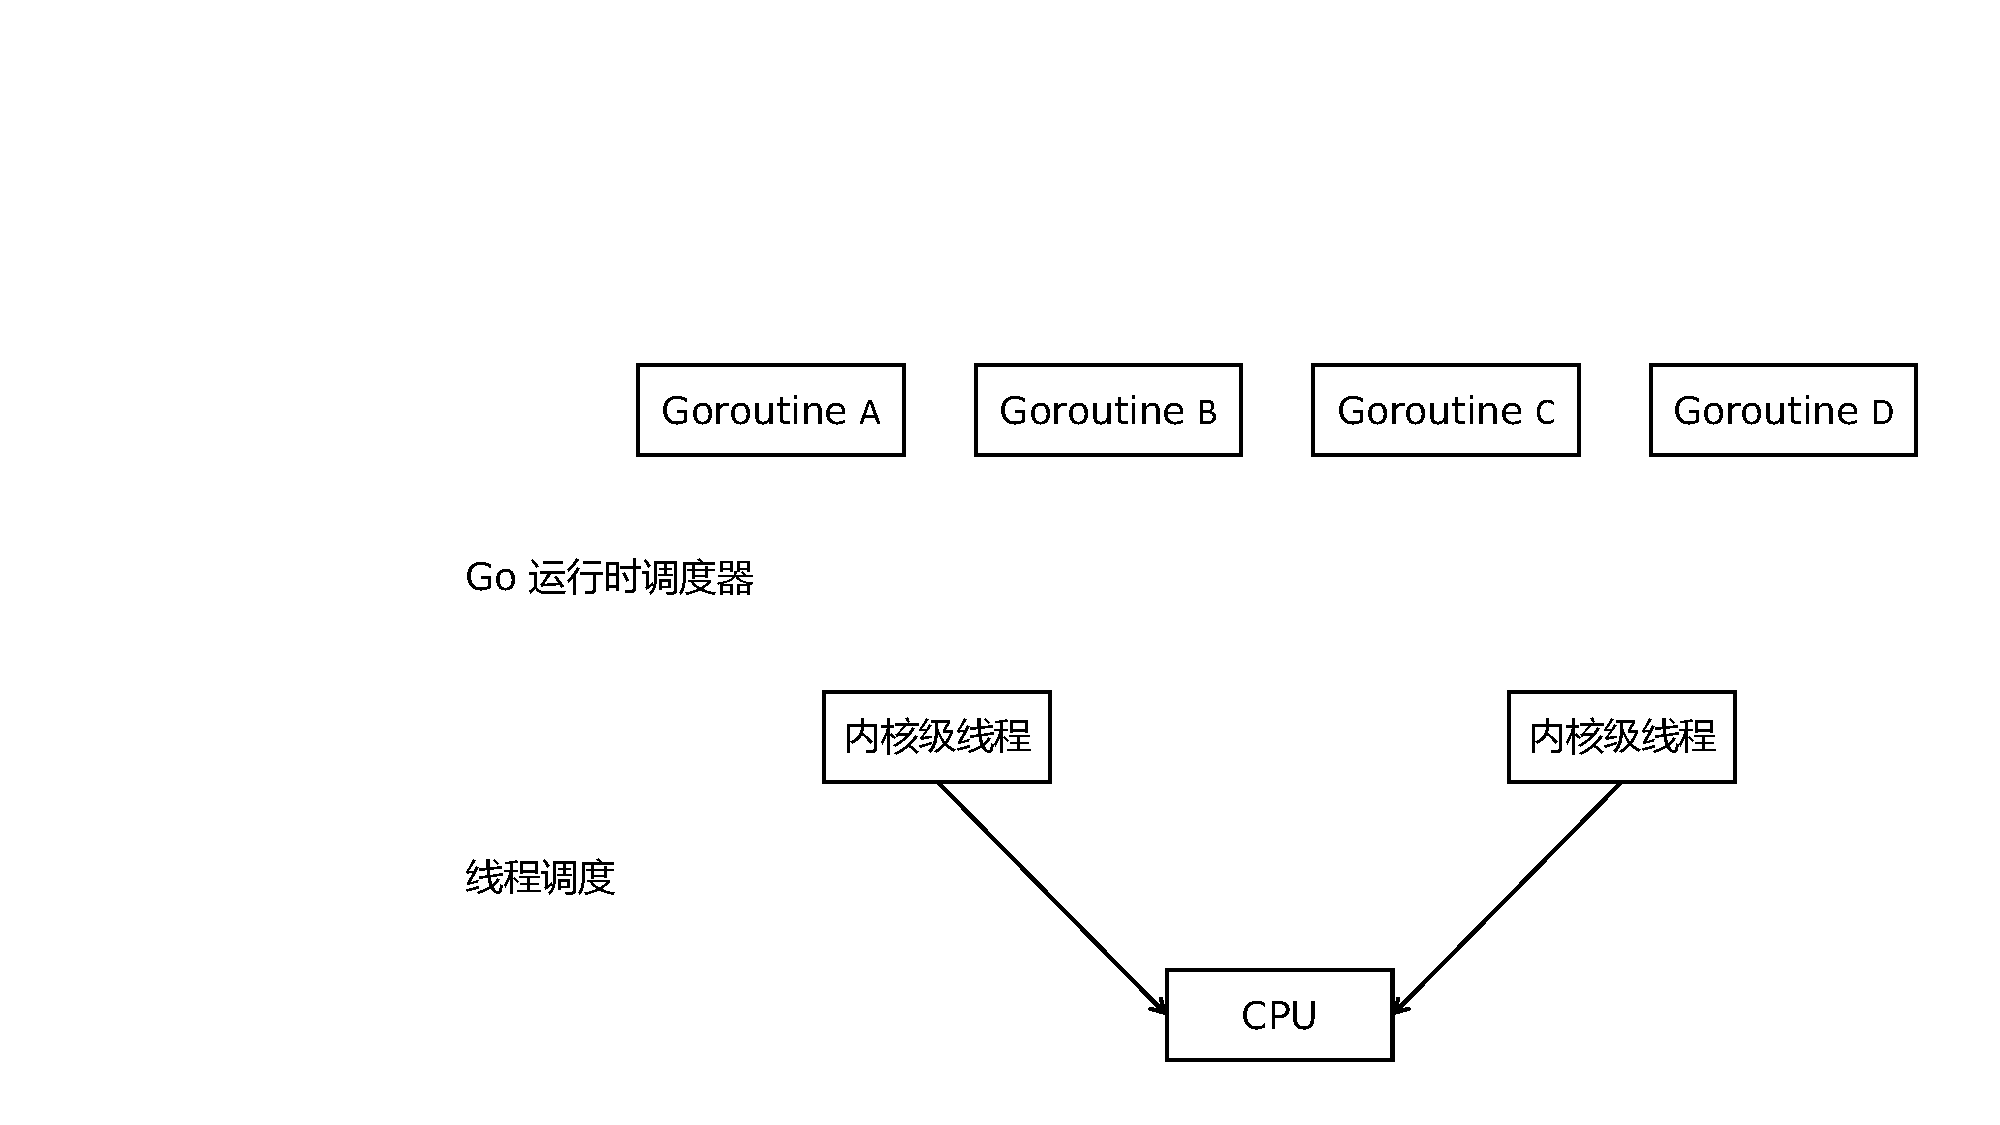
\includegraphics[width=13cm]{images/fig1.pdf}
                \caption{条件假设}
                \label{fig1}
            \end{figure}
        \item 现假设出于某些原因,Go 的运行时调度程序决定如图\ref{fig2}这样将 Goroutines 多路复用到线程上. Goroutine A 和 B 将使用左侧的内核线程运行,Goroutines C 和 D 将使用右侧的内核线程运行,同时假设 Goroutines 将从放置在 Goroutines 池底部的 Goroutine 开始分别运行.
            \begin{figure}[!htbp]
                \centering
                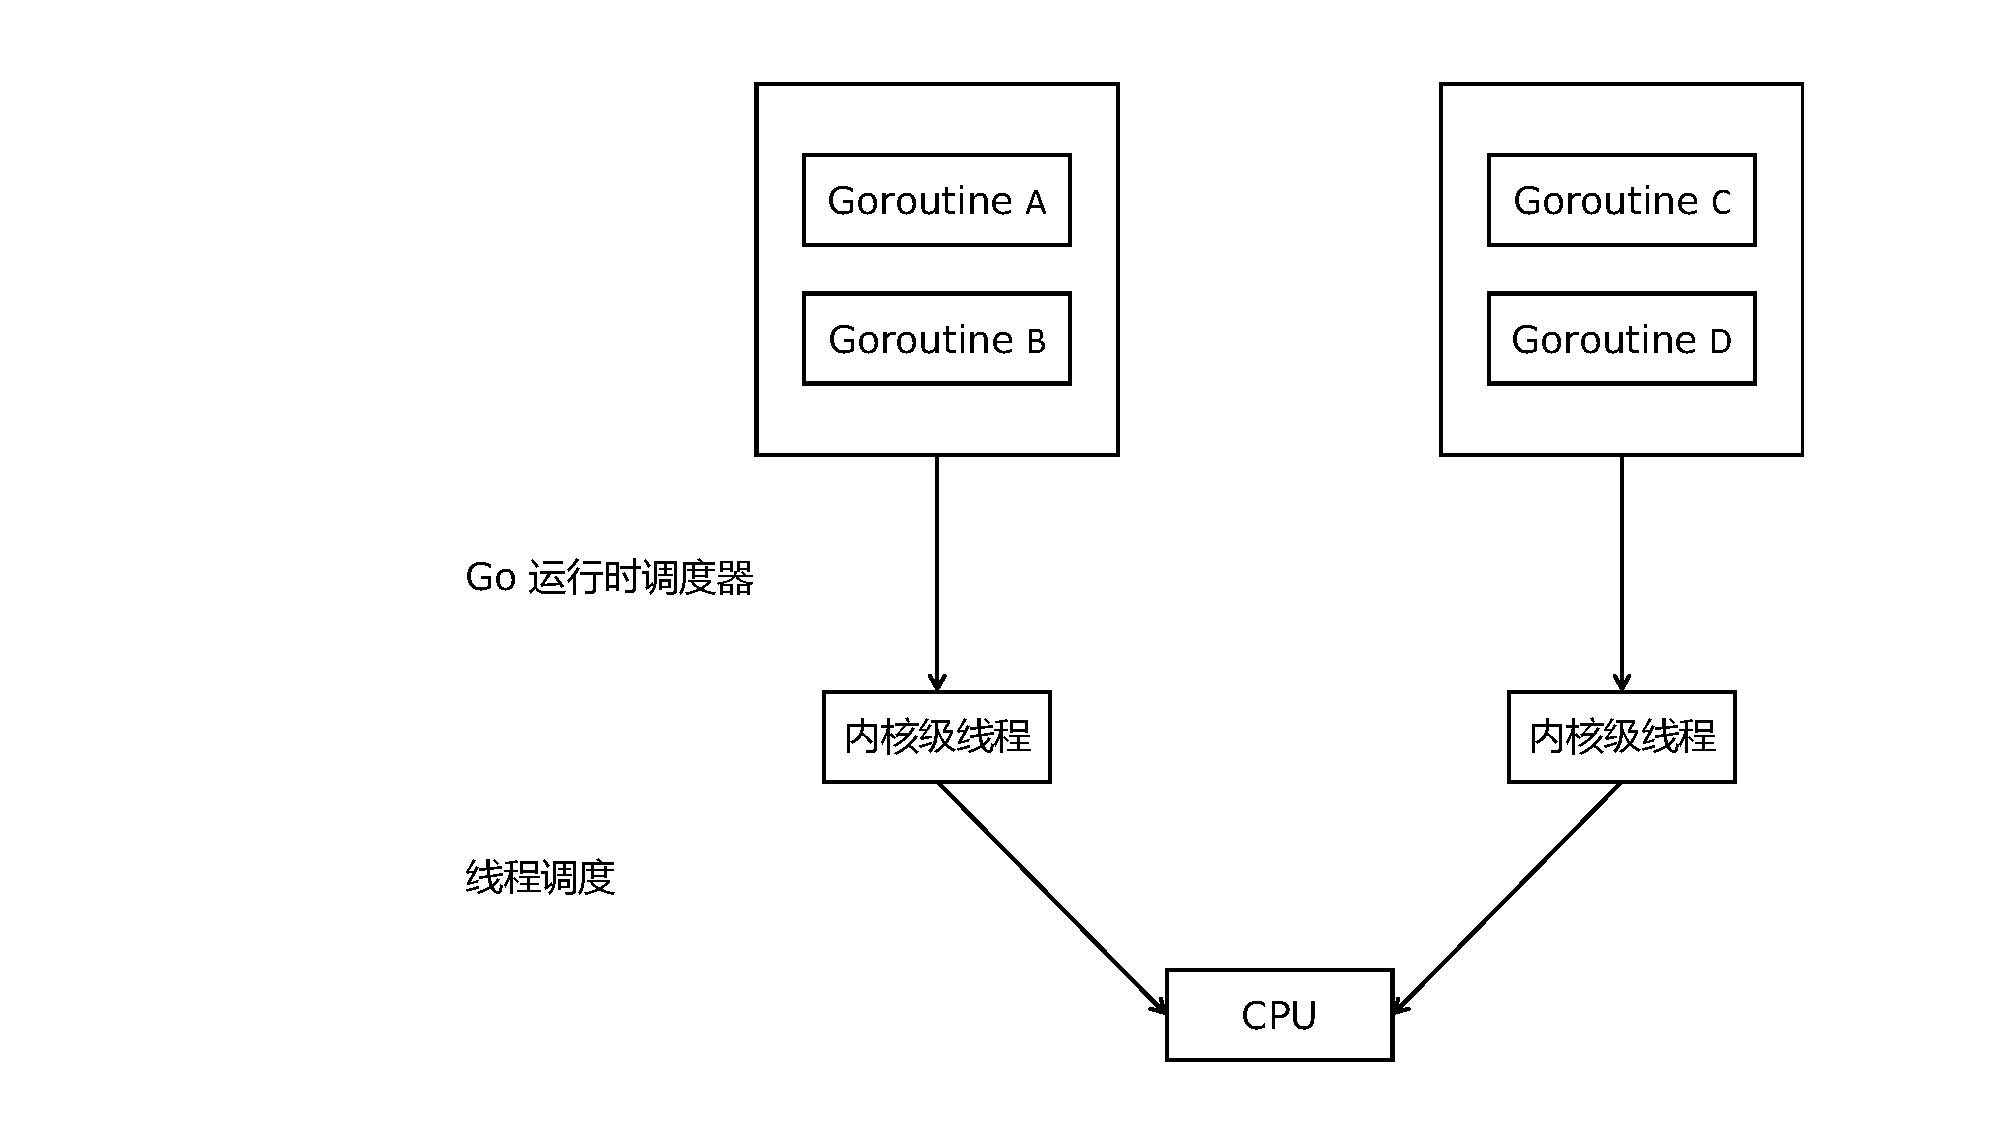
\includegraphics[width=13cm]{images/fig2.pdf}
                \caption{初始情况}
                \label{fig2}
            \end{figure}
        \item 现在 Goroutines 开始运行。但此时 “A” 调用了一个阻塞的系统调用(例如 read() 语句),导致 Goroutine A 处于阻塞中,Goroutine B 被阻塞.
            \begin{figure}[!htbp]
                \centering
                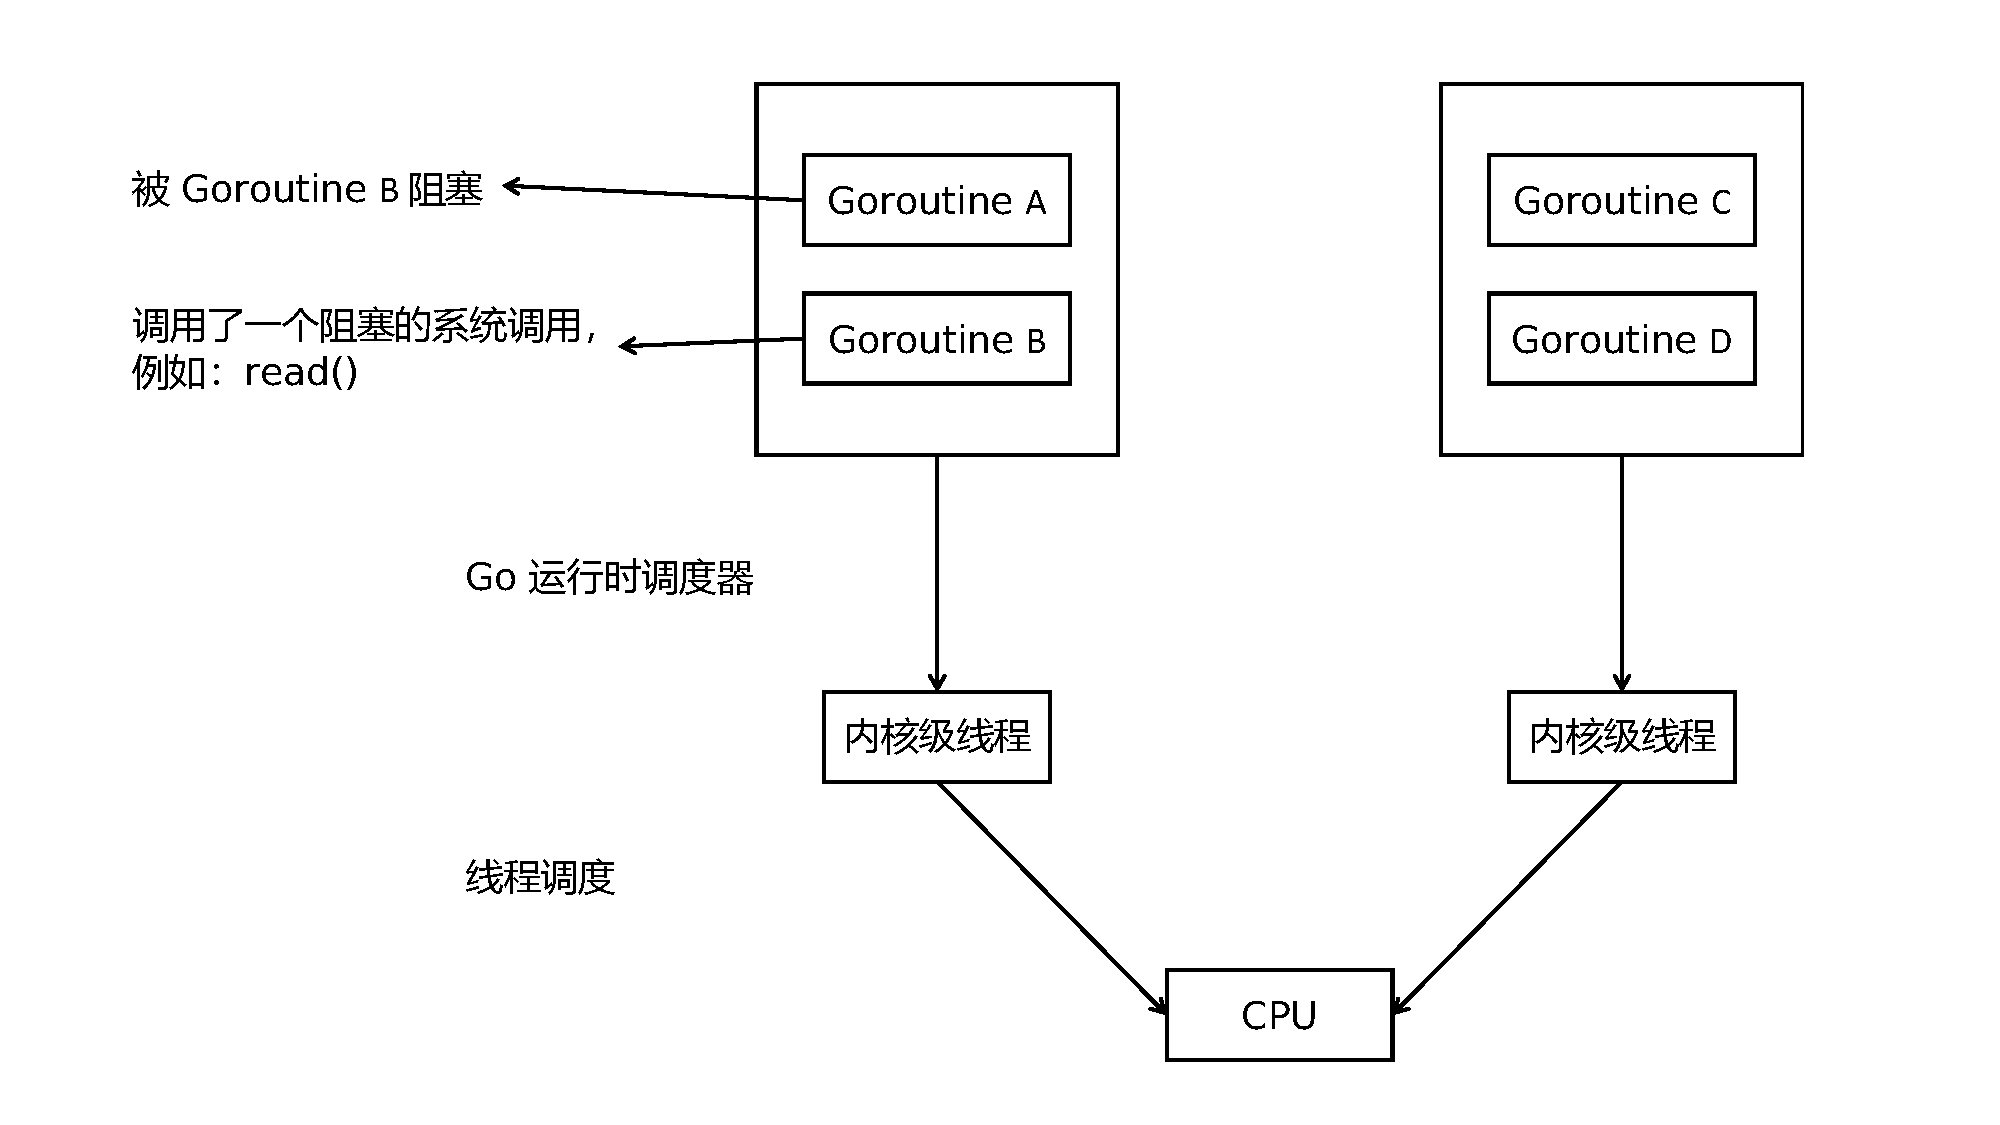
\includegraphics[width=13cm]{images/fig3.pdf}
                \caption{阻塞出现}
                \label{fig3}
            \end{figure}
        \item Goroutine D 已经执行完毕.
            \begin{figure}[!htbp]
                \centering
                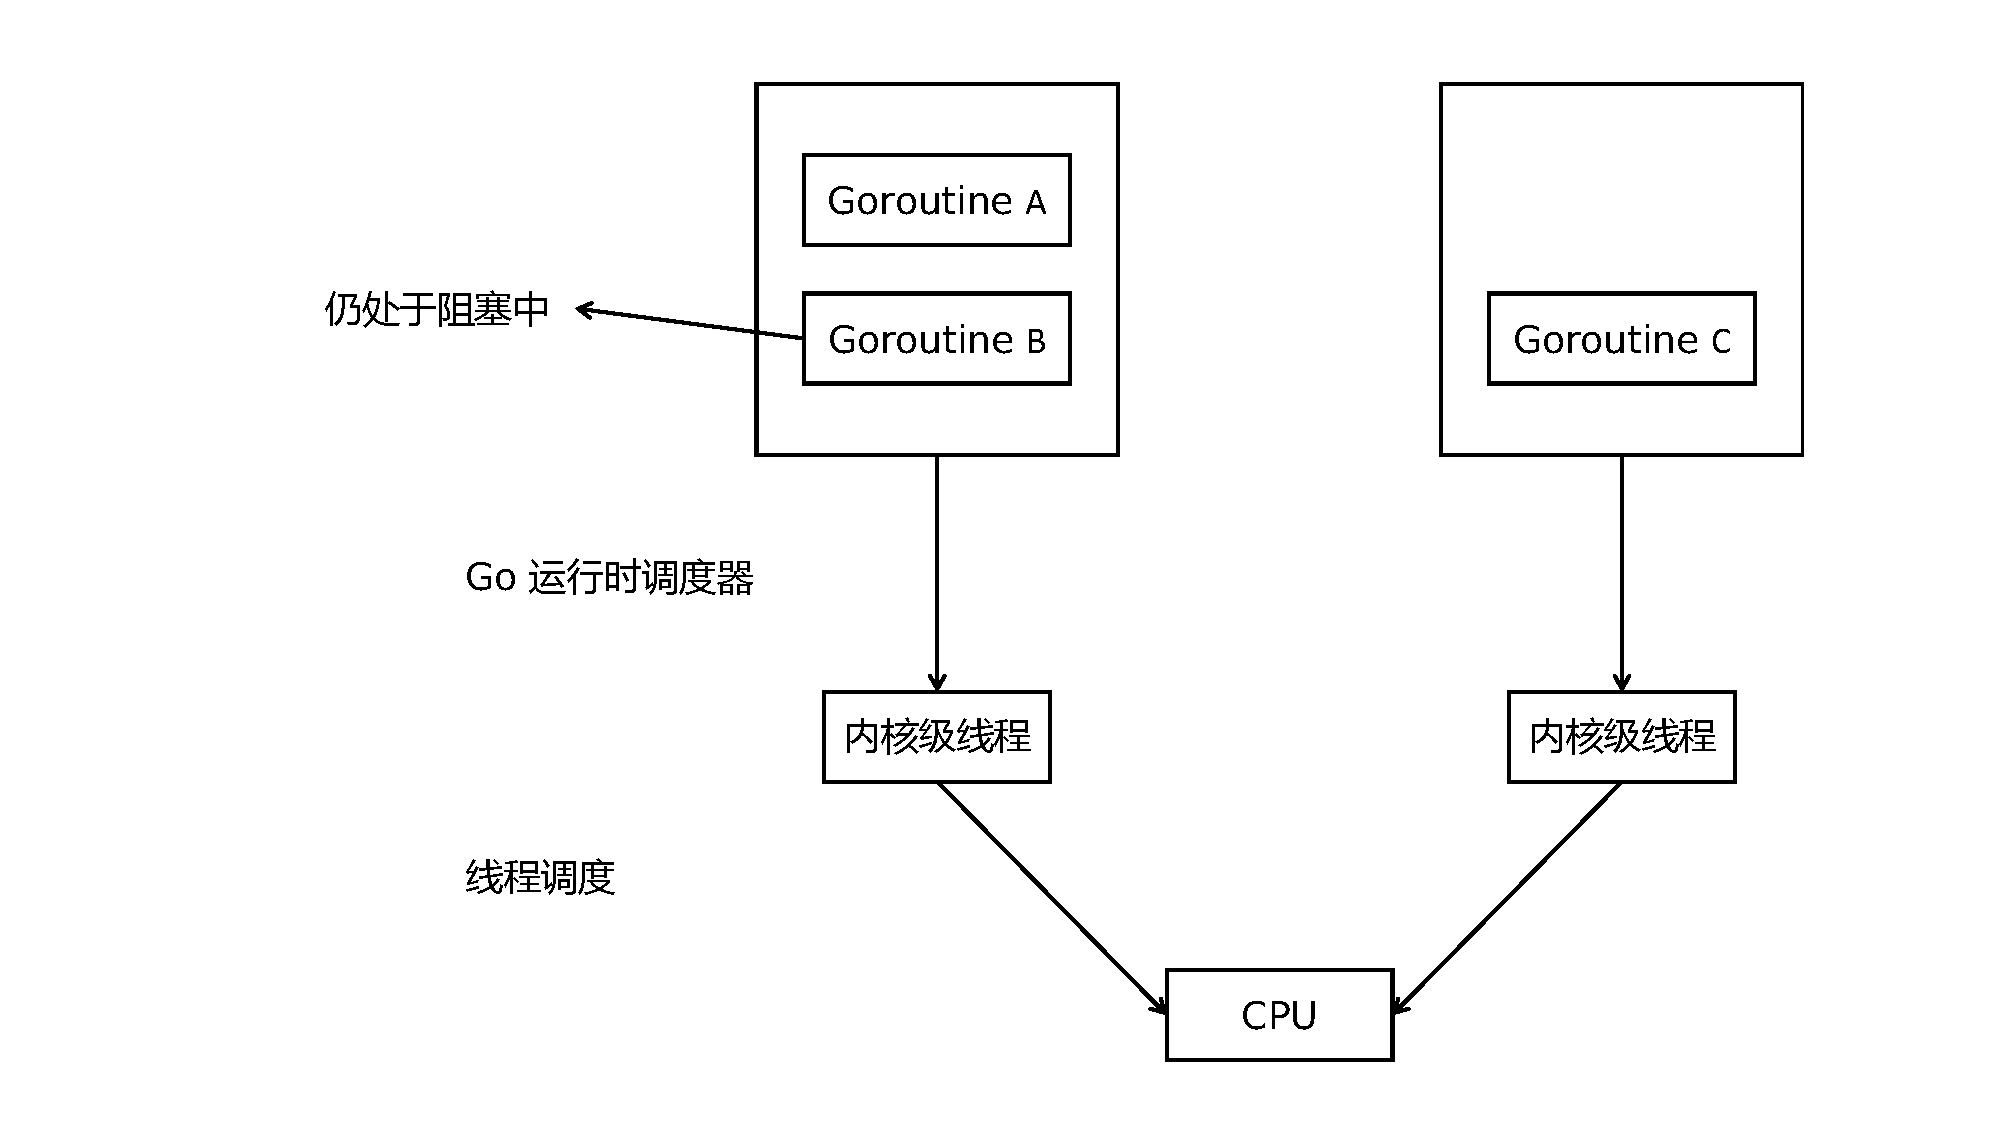
\includegraphics[width=13cm]{images/fig4.pdf}
                \caption{Goroutine D 执行完毕}
                \label{fig4}
            \end{figure}
        \item Go 的运行时调度程序现在可能会意识到,将 Goroutine A 移动到另一个可运行线程而不是永远等待 Goroutine B 执行完毕会是一个更好的主意.
            \begin{figure}[!htbp]
                \centering
                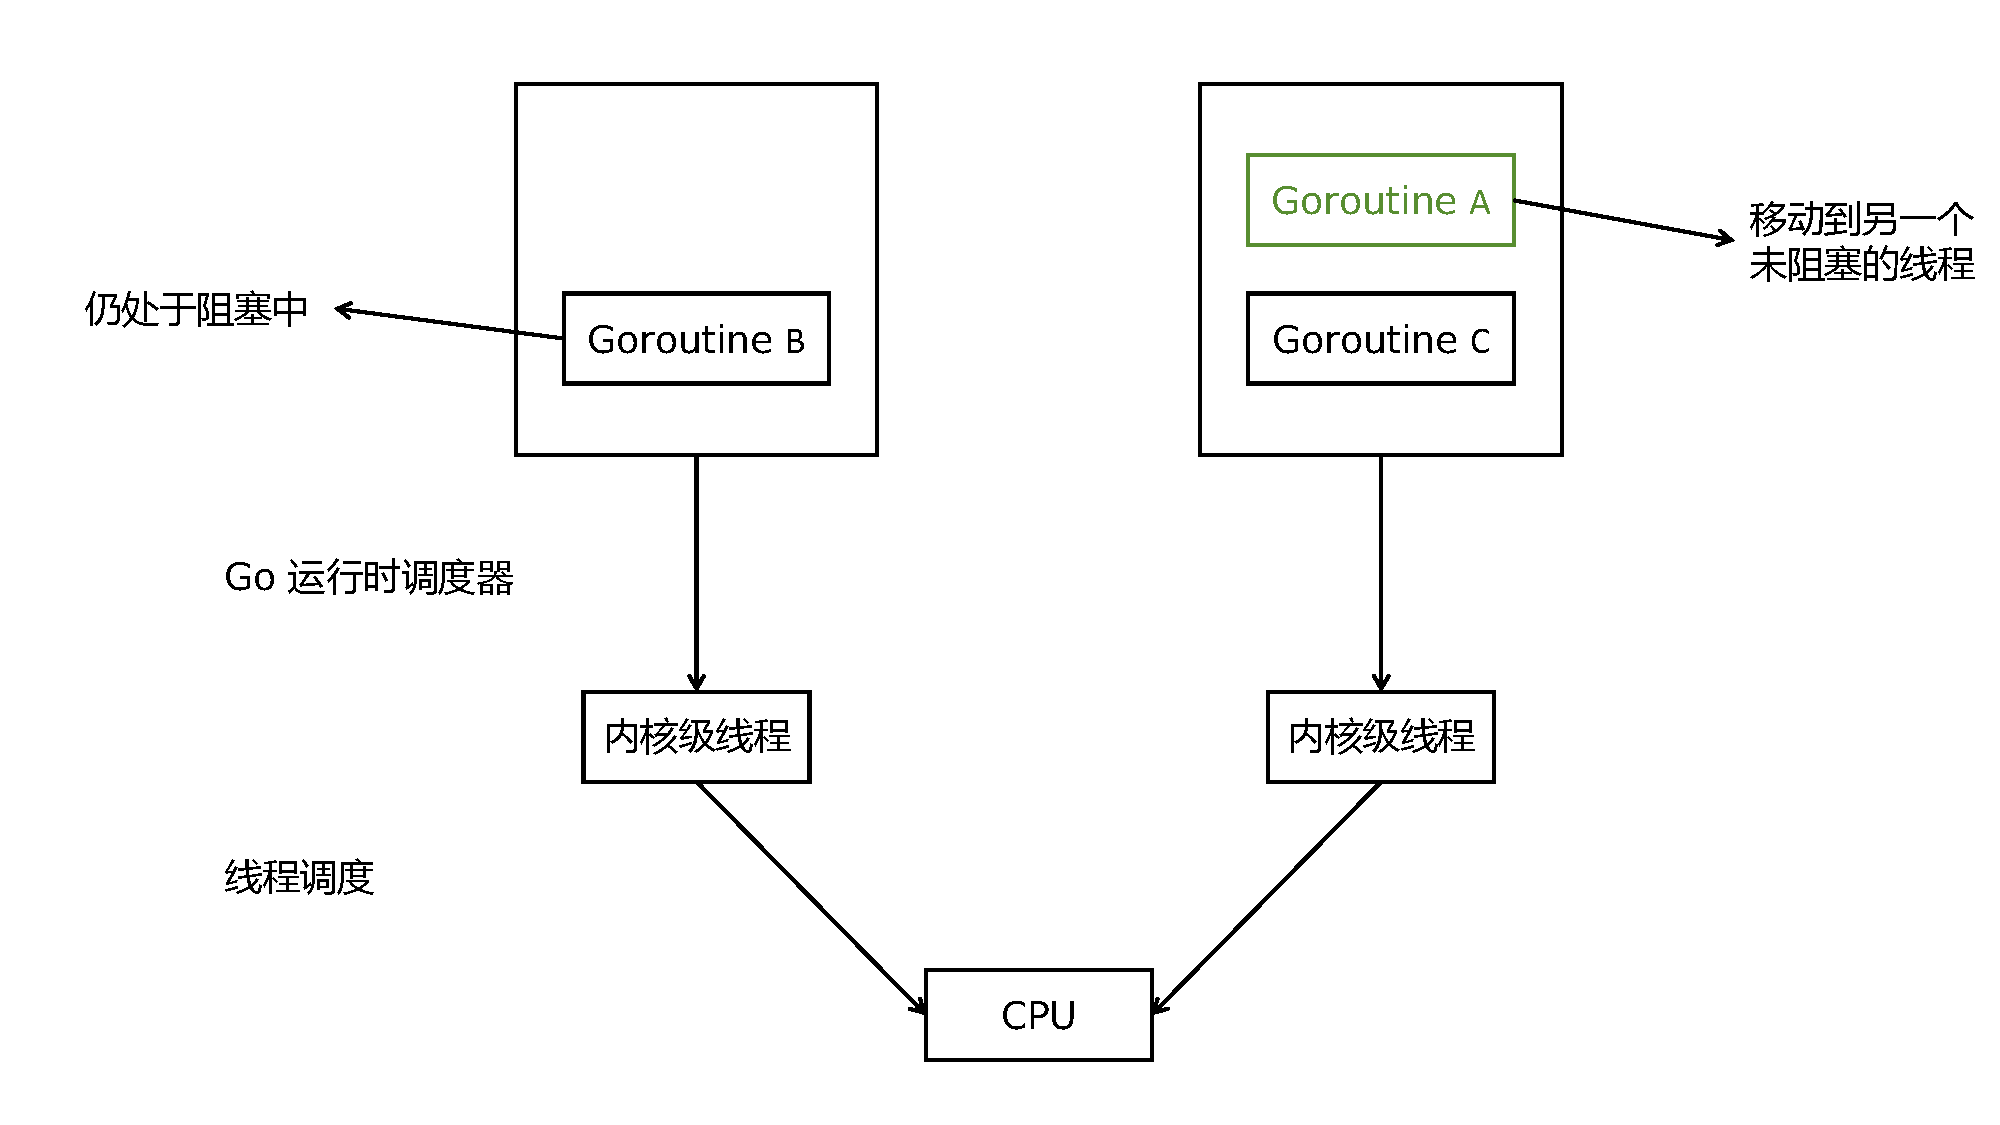
\includegraphics[width=13cm]{images/fig5.pdf}
                \caption{将 B 移动到另一个 Goroutine 池}
                \label{fig5}
            \end{figure}
            \newpage
        \item Goroutine C 现在已经执行完毕.
            \begin{figure}[!htbp]
                \centering
                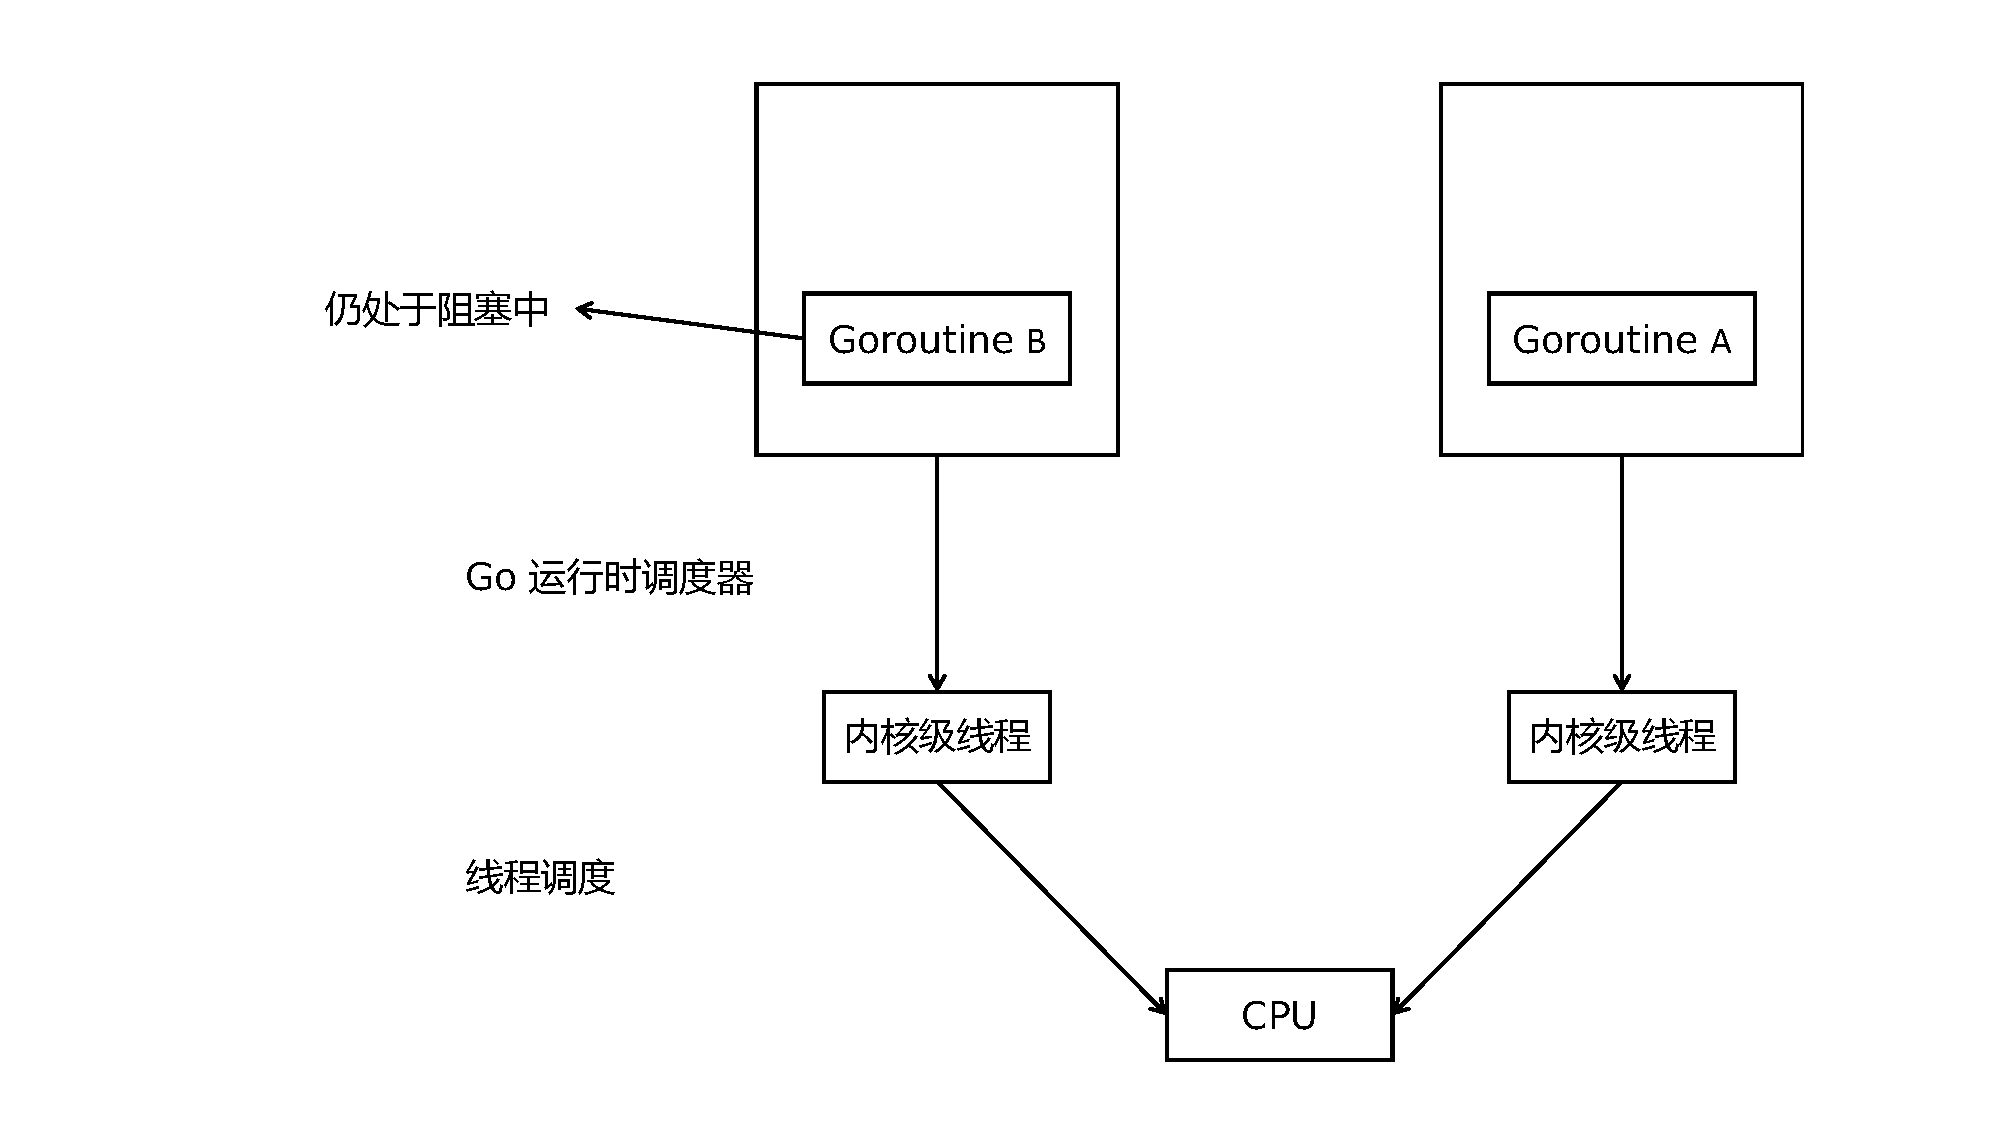
\includegraphics[width=13cm]{images/fig6.pdf}
                \caption{Goroutine C 执行完毕}
                \label{fig6}
            \end{figure}
        \item Goroutine A 现在也完成了,而左边被 Goroutine B 占用的内核线程还处于阻塞中的状态.
            \begin{figure}[!htbp]
                \centering
                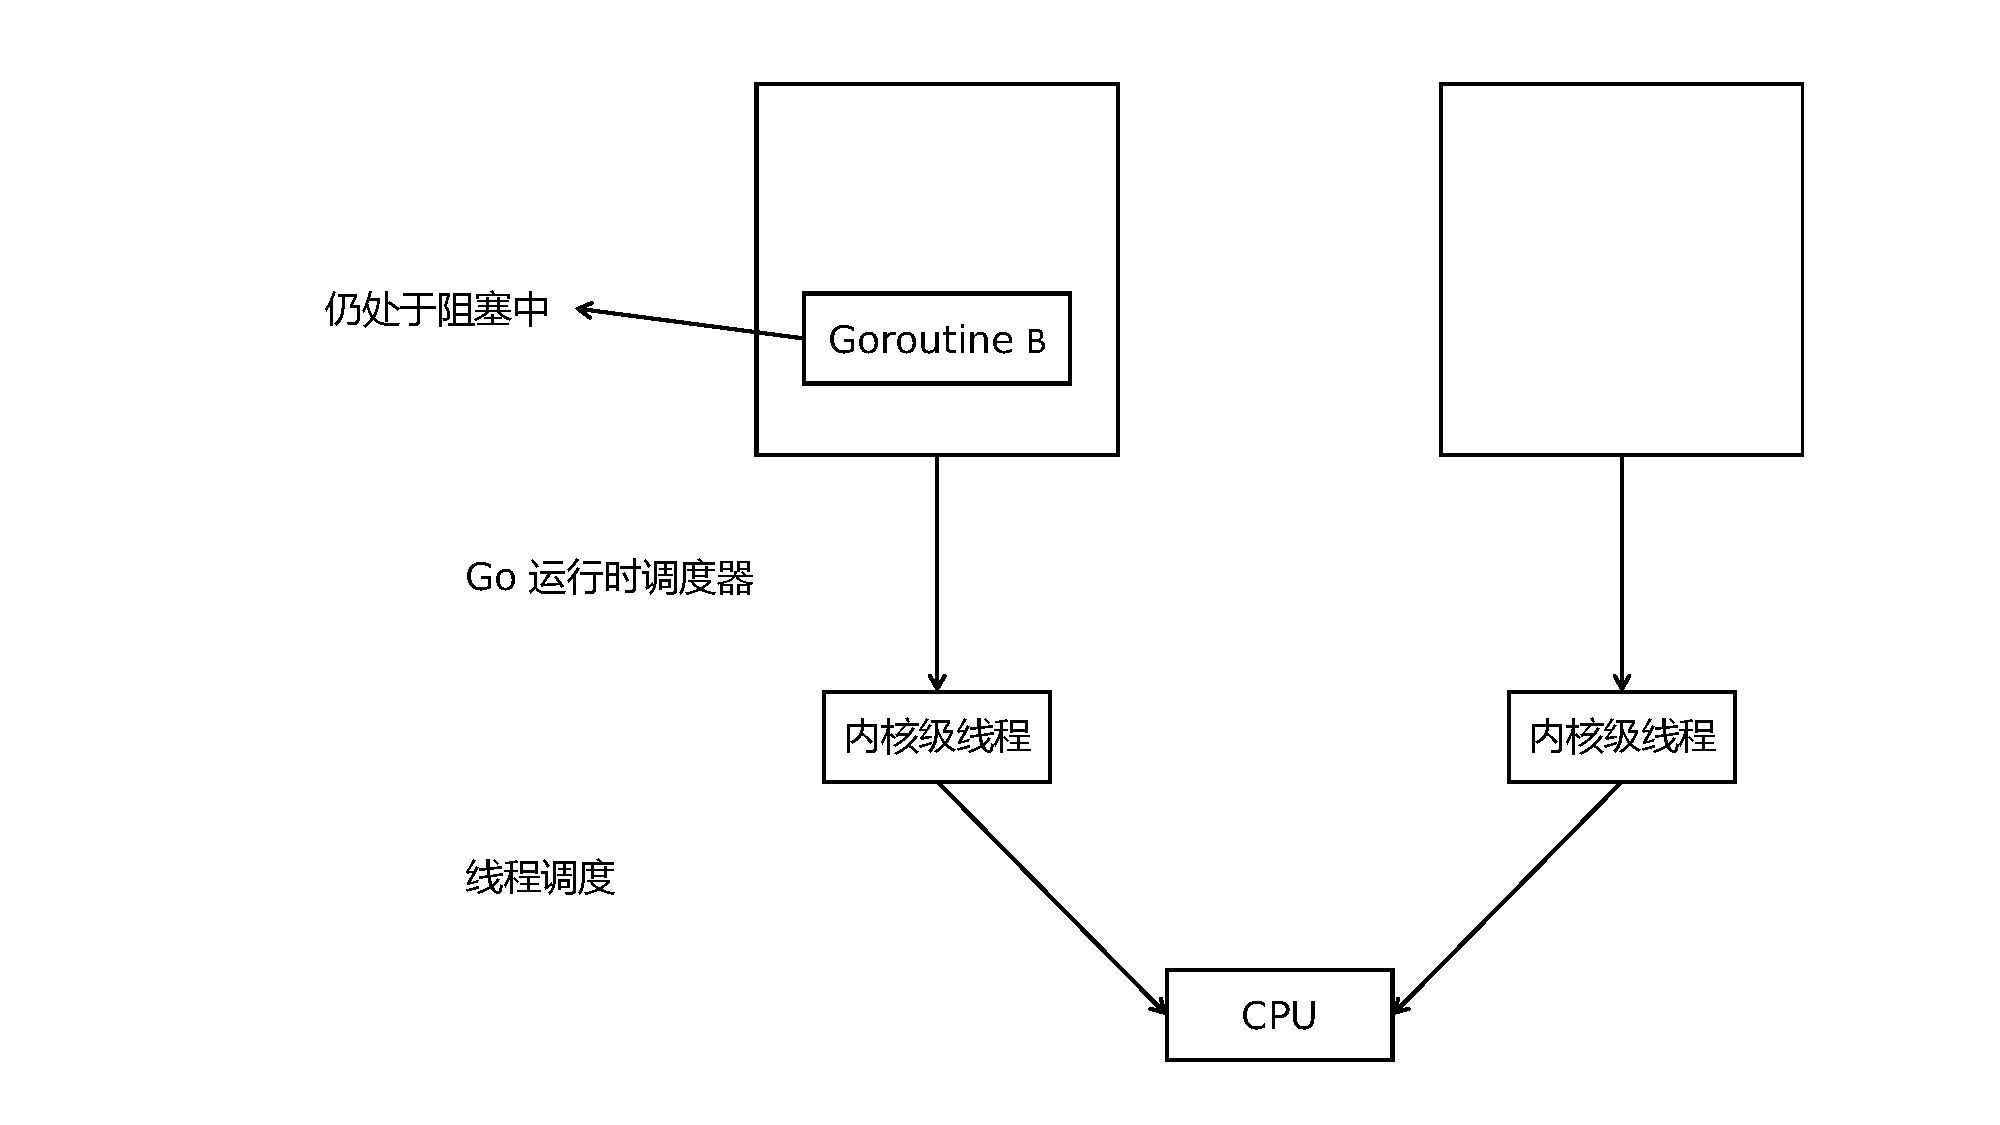
\includegraphics[width=13cm]{images/fig7.pdf}
                \caption{Goroutine A 执行完毕}
                \label{fig7}
            \end{figure}
    \end{itemize}
    \newpage
    如果 Go 运行时调度器没有将阻塞的 Goroutine 重新调度到另一个可运行的线程,那么 Goroutine A 到现在仍然不会被执行.
\end{solution}

\end{document}